\chapter{Physical Sensing}

The successful application of machine learning methods demands comprehensive, carefully curated data sets. In order for our modeling efforts to be successful, it is critical that we capture the subtle nuances of the phenomena we wish to describe. In this chapter, we outline the various physical sensing approaches used throughout this dissertation, all of which are part of a broader effort in the MINTS-AI laboratory at the University of Texas at Dallas. MINTS-AI is an acronym for, Multi-Scale Multi-Use Integrated Intelligent Interactive Sensing in Service of Society for Actionable Insights. An graphical overview of the MINTS-AI sensing paradigm is described in Figure \ref{fig:mints-ai}.

\begin{figure}[!hbt]
  \centering
  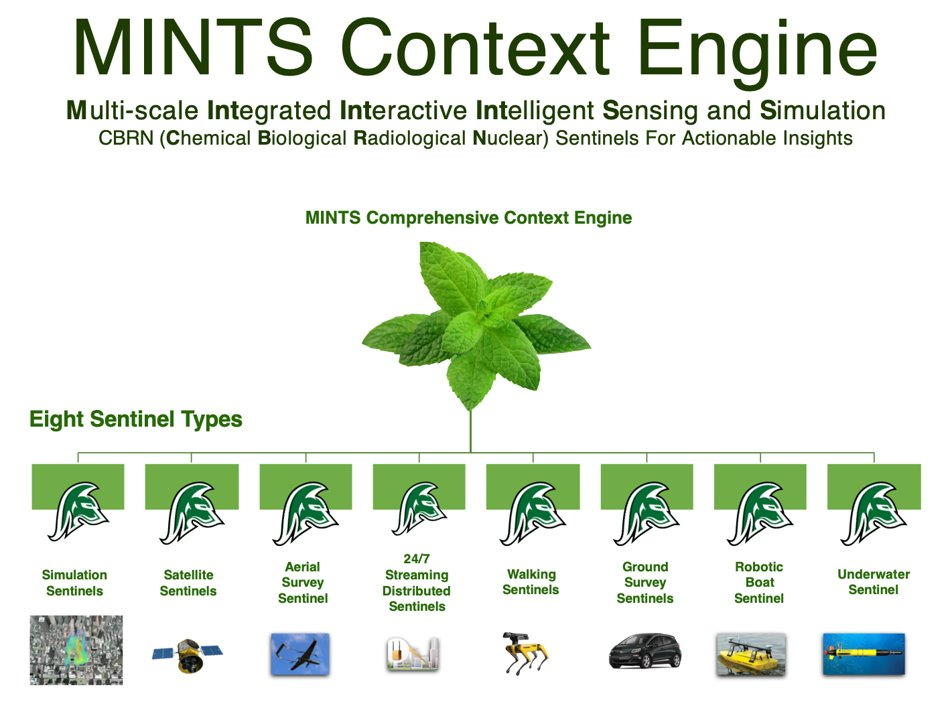
\includegraphics[width=0.8\textwidth]{physical-sensing/MINTS-sentinels.jpg}
  \caption{The MINTS-AI context engine is a sensing paradigm composed of flexible sensing sentinels spanning from remote sensing data products to autonomous robots and ground survey vehicls.}
  \label{fig:mints-ai}
\end{figure}

Of the variety of sensing sentinels outlined above, this dissertation is primarily concerned with three key applications. The first is a team of autonomous robotic vehicles which we refer to as the \textit{robotic team}. The second is a network of distributed streaming sentinels comprised of low-cost air quality sensors. The third describes a reference sensor chamber for air quality evaluation which we use to develop a \textit{simulation sentinel}.


% -------------------------------------------------------------------- %

\section{Coordinated Robotic Teams}

Recent developments in hyperspectral imaging technology have led to dramatic reductions in both size and weight of imaging platforms. Due to these improvements, it is now possible to incorporate the technology as the payload of highly mobile autonomous aerial vehicles such as drones. However, the massive volume of hyperperspectral datacubes poses significant computational challenges to their adoption in real-time applications. For decades, multi-spectral imagers have seen wide spread adoption in the remote sensing community as a means to take advantage of the wealth of information contained in the reflectance spectra of materials. In addition to the three color filters of traditional cameras, \textit{multi-spectral} imagers, like those deployed on MODIS, Sentinel 2, and other satellite missions, capture many additional features by utilizing wavelength bands ranging from the near-UV, through the visible spectrum, and into the Infrared. With this additional information, multi-spectral remote sensing platforms are able to aid in a variety of domains from tracking land change, characterizing deforestation, monitoring erosion, evaluating crop health, and many others (add reference).

\begin{figure}[!hbt]
  \centering
  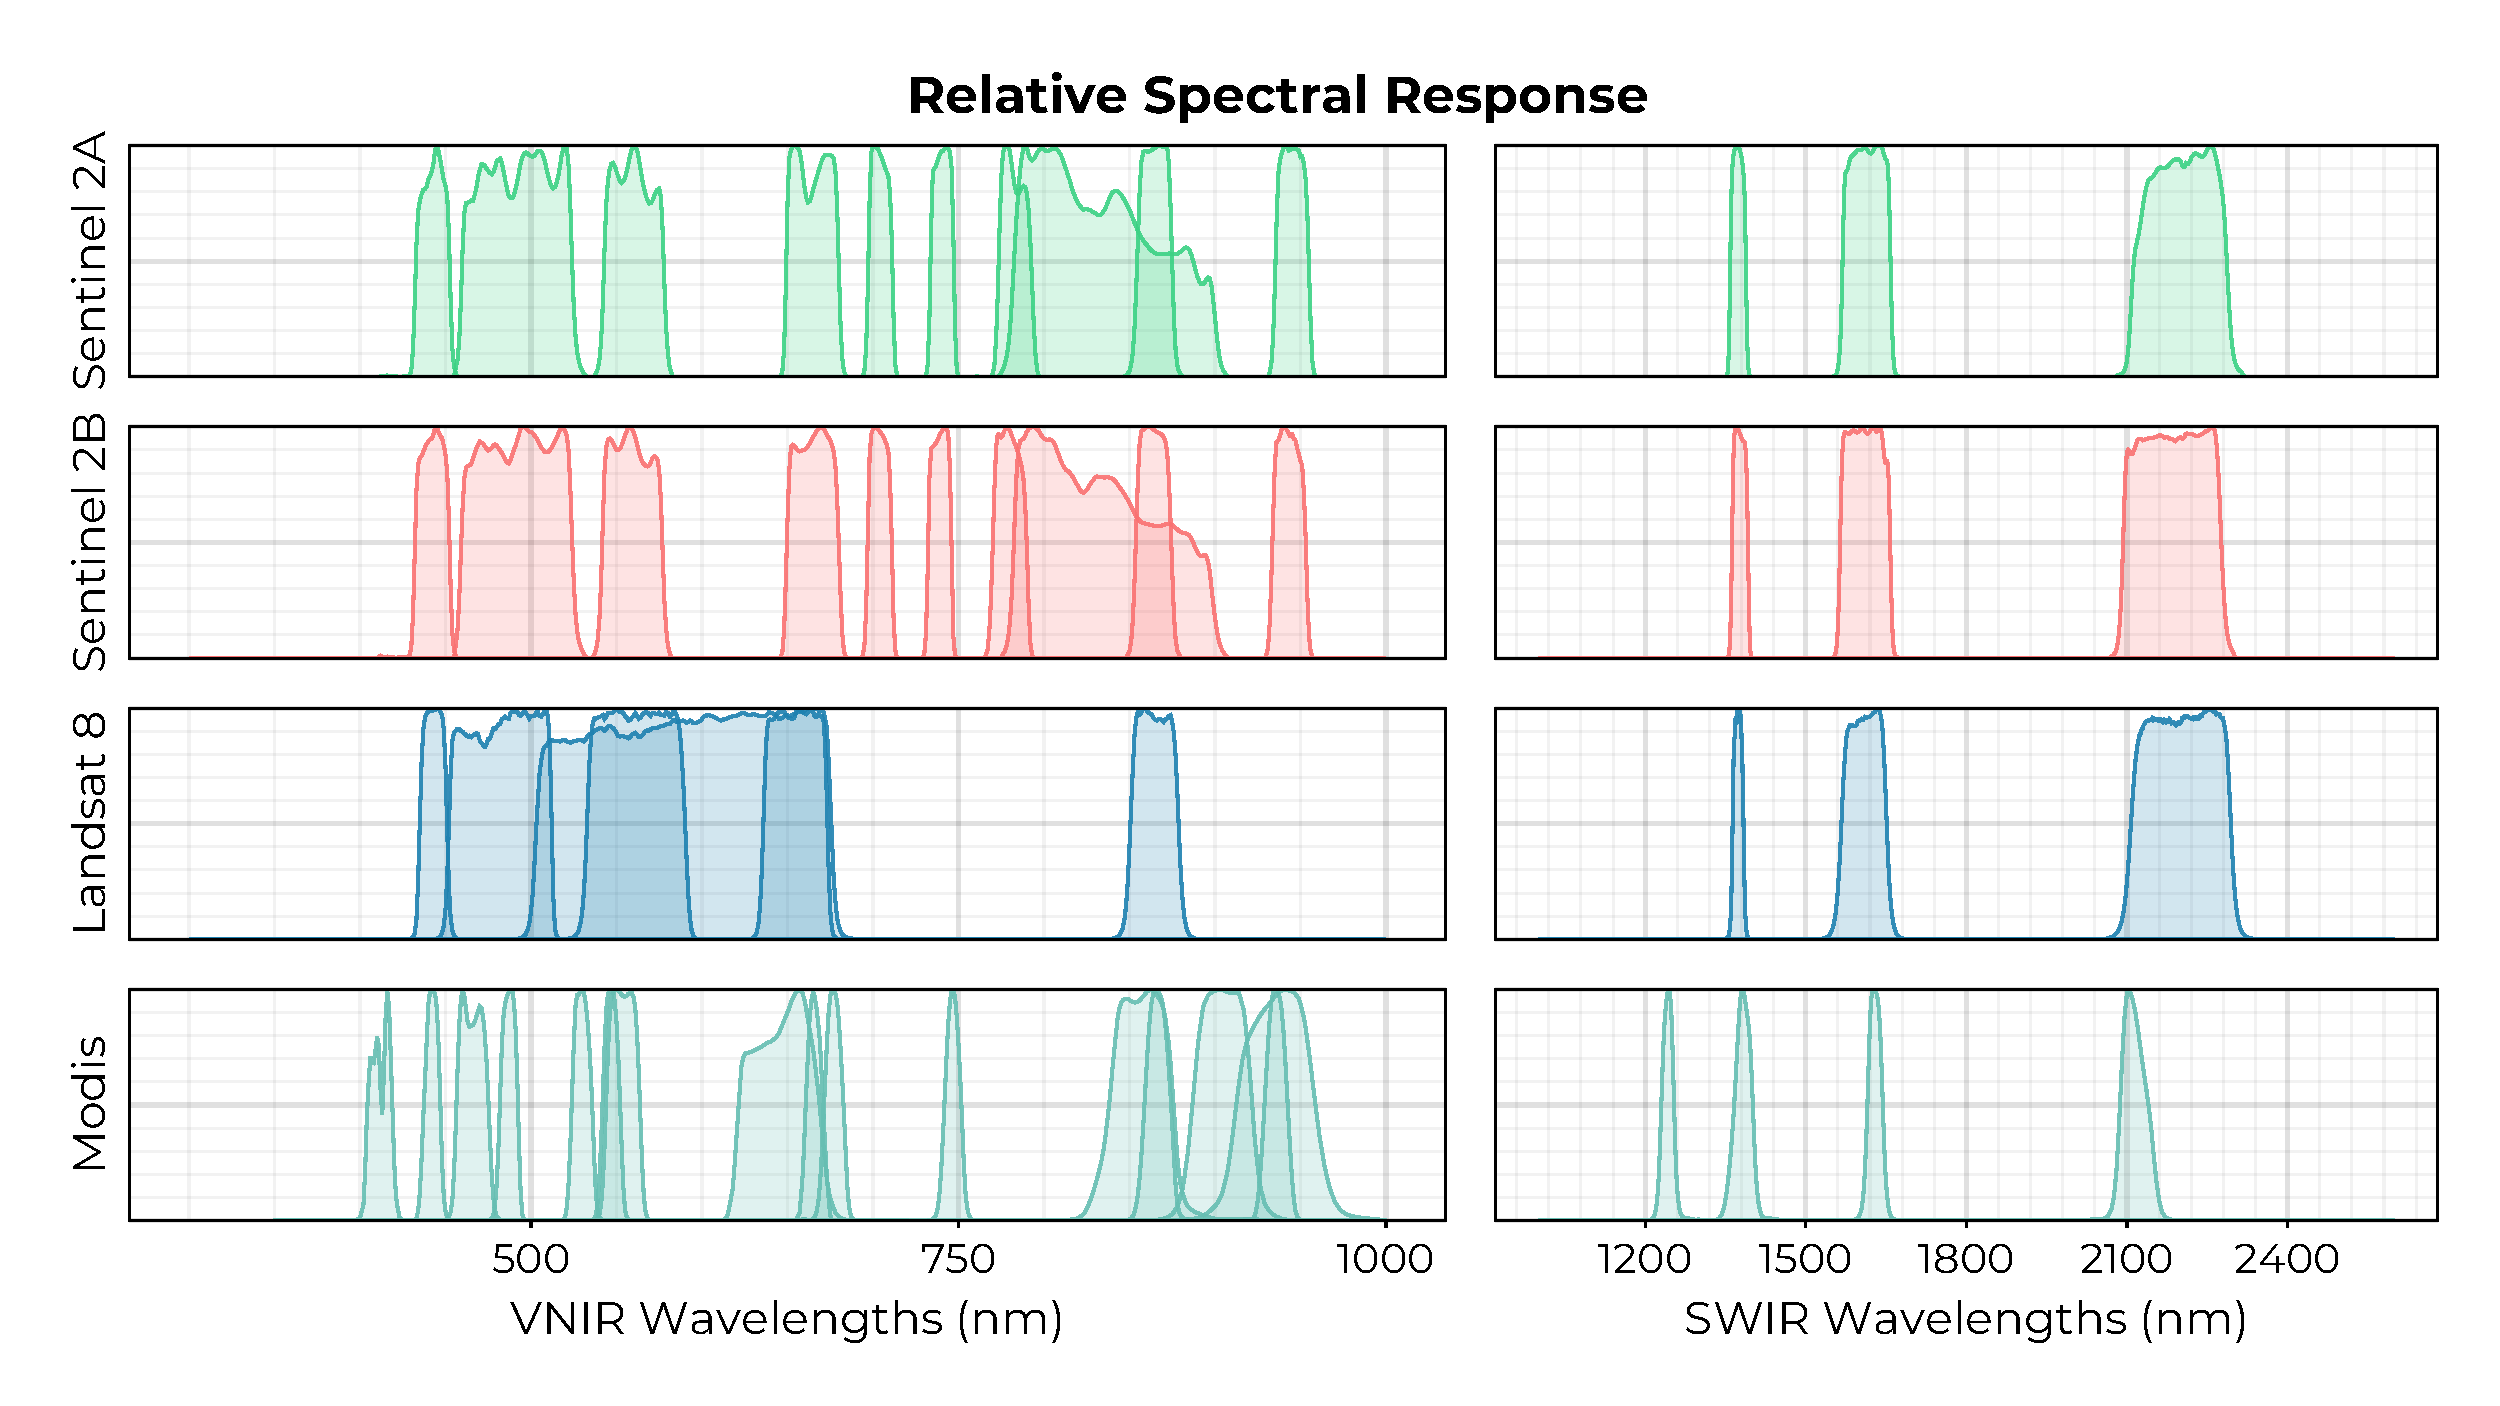
\includegraphics[width=0.85\columnwidth]{robot-team/assets/passbands.pdf}
  \caption{A comparison of the relative spectral response for the passbands of popular multi-spectral imaging remote sensing platforms.}
  \label{fig:passbands}
\end{figure}

These uses are justified by the reflectance features of materials across the electromagnetic spectrum; water has vibrational modes in the infrared while pigments tend to have absorption peaks in the visible portion of the spectrum. Many currently used spectral indices like the normalized difference vegatation index (NDVI) take advantage of these spectral regions by comparing ratios of pigment sensitive passbands to the stable signals in the infrared to infer the abundance of chlorophyll, and consequently, the health of plants.  However, despite the plethora of successful applications of multi-spectral imaging, more can be accomplished with the additional information provided by fully resolved spectra. For example, in the laboratory, spectrophotometry allows the direct determination of the concentrations of chemicals constituents in solution by deconvolution of a sample spectrum against libraries of carefully collected of reference spectra: individual chemicals be uniquely identified by the characteristic location and shape of their absorption features.

At the terrestrial level, drones (commonly, quadcopters, octocopters, and other similar multi-rotor craft) equipped with cameras are able to utlize techniques of photogrametry together with continuously sampled imagery to produce high quality digital elevation maps, high quality mosaics, 3-dimensional reconstructions, etc. These capabilities provide significant aid for structural analysis and smart agriculture to name a few applications. Today, kilogram-scale HSI can be comfortably mounted to the payload of drones such as the AltaX and advancements in spectral sensing such as (reference Ethan Minot's recent paper) suggest that sizes of HSI will continue to shrink further expanding their application in this domain.

The inspiration for this autonomous robotic team is the automation of what is currently done manually in the production of remote sensing satellite data products. The typical timescale from starting work on a new remote sensing data product to its operational readiness is at least a couple of years, but, more typically, a decade or more. A key part of this substantial time delay is due to the time that is taken for the collection of the relevant training data. Hence, our goal is to reduce this timescale to be near real time by utilizing an autonomous robotic team that can both collect the training data, and then in real time process and stream the remote sensing data products. The fully autonomous team includes a robotic boat that carries a suite of sensors to measure in-situ water composition in real time as well as a sonar, and an autonomous UAV equipped with a down-welling irradiance spectrometer, hyper-spectral, and thermal imagers, together with an onboard Machine Learning (ML) capability. Figure \ref{fig:drone-team} shows photographs of the robot team during a deployment in North Texas.

\begin{figure}[!hbt]
  \centering
  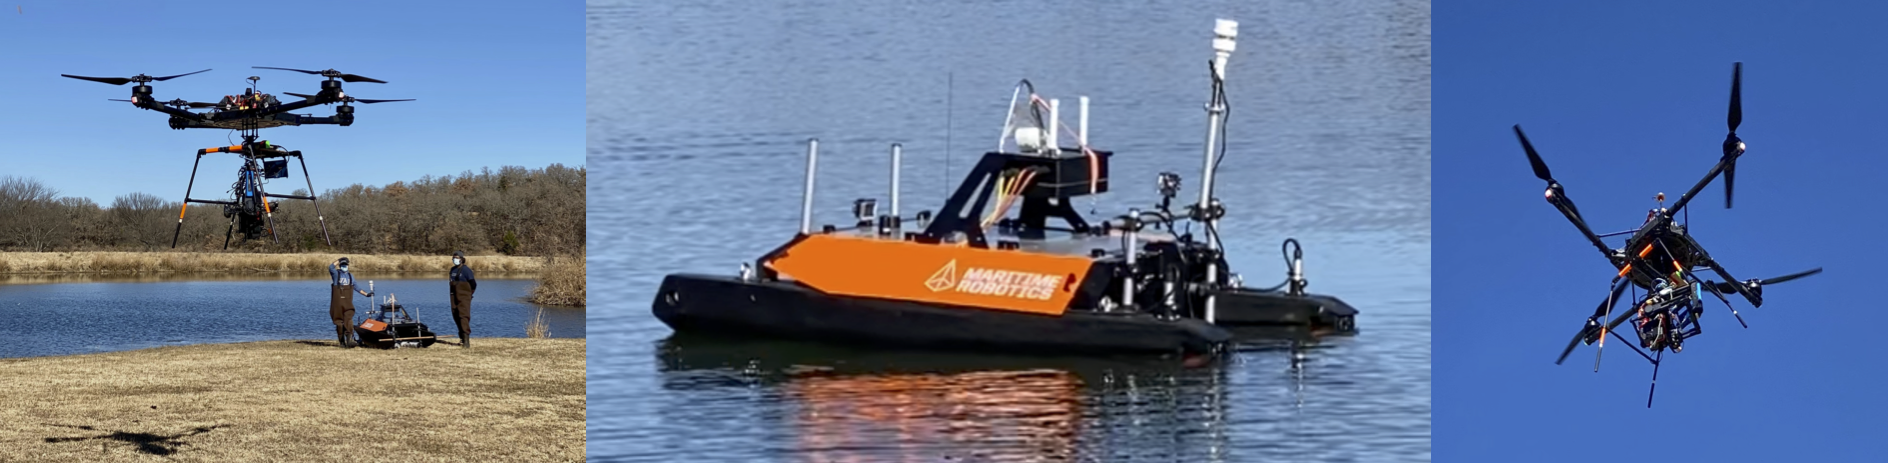
\includegraphics[width=0.9\columnwidth]{physical-sensing/Photos.png}
  \caption{The MINTS robotic team}
  \label{fig:drone-team}
\end{figure}

The autonomous boat used is a \href{https://www.maritimerobotics.com/otter}{Maritime Robotics Otter }. With a footprint of only 200 × 108 × 81.5 cm, a weight of 55 kg, and dual electrical fixed thrusters, it is an easily deployable asset that can be transported in a van or even within normal airliners to a survey site. With a cruise speed of two knots, it has a duration of 20 h from one charge of the batteries. It can use WiFi, cellular, and an optional AIS receiver for communication to the control station. Our drone is a \href{https://freeflysystems.com/alta-x}{Freefly Alta-X} professional quad-copter. It was specifically designed to carry cameras, with a payload capacity of up to 35 lb, a long range data link, and autonomy provided by the Open PX4 flight stack. The open source QGroundControl software was used to control the autonomous operations.

All of the robotic team members carry a high-accuracy GPS and inertial navigation system (INS), so that every data point can be geo-located and time stamped. Each of the robots can also join the same network which connects the robots and their ground-control stations. Our robots use long-range \href{https://www.ui.com}{Ubiquiti 5 GHz LiteBeam airMAX WiFi}. This network also includes a local \href{https://www.synology.com}{Synology network-attached storage (NAS)} device in the robot team control trailer, which, in real-time, syncs the data that are collected to the NAS in our home laboratory at the university. 

The robotic boat payload included a \href{https://www.biosonicsinc.com/products/mx-aquatic-habitat-echosounder/}{BioSonics MX Aquatic Habitat Echosounder sonar} for rapid assessment and mapping of aquatic vegetation, substrate and bathymetry. Three \href{https://www.waterprobes.com/multiprobes-and-sondes-for-monitori}{Eureka Manta-40 multi-probes}, a \href{https://www.sequoiasci.com/product/lisst-abs/}{Sequoia Scientific LISST-ABS acoustic backscatter sediment sensor}, and an \href{https://www.airmar.com/weather-description.html?id=153}{Airmar Technology Corporation 220 WX ultra-sonic weather monitoring sensor}.

The first Manta-40 multi-probe included sensors for temperature and turbidity and \href{https://www.turnerdesigns.com/cyclops-7f-submersible-fluorometer}{Turner Designs Cyclops-7 submersible Titanium body fluorometers} for Chlorophyll A, Chlorophyll A with Red Excitation, Blue-Green Algae for fresh water (Phycocyanin), Blue-Green Algae for salt water (Phycoerythrin), and CDOM/FDOM. The second Manta-40 multi-probe included sensors for temperature, conductivity (with specific conductance, salinity, and total dissolved solids, TDS), pH (with separate ref-
erence electrode), optical dissolved-oxygen, turbidity, and Ion Selective Electrodes by Analytical Sensors and Instruments (http://www.asi-sensors.com/, accessed 05/01/2021)
for ammonium ($\mathrm{NH_4^+}$), bromide ($\mathrm{Br^−}$), calcium ($\mathrm{Ca^{2+}}$), chloride ($\mathrm{Cl^−}$), nitrate ($\mathrm{NO_3^{-}}$), and sodium ($\mathrm{Na^+}$). The third Manta-40 multi-probe included sensors for temperature, turbidity, a total dissolved gas sensor, and Turner Designs Cyclops-7 submersible Titanium body fluorometers for optical brighteners, crude oil, refined fuels, and tryptophan.

\begin{figure}[!hbt]
  \centering
  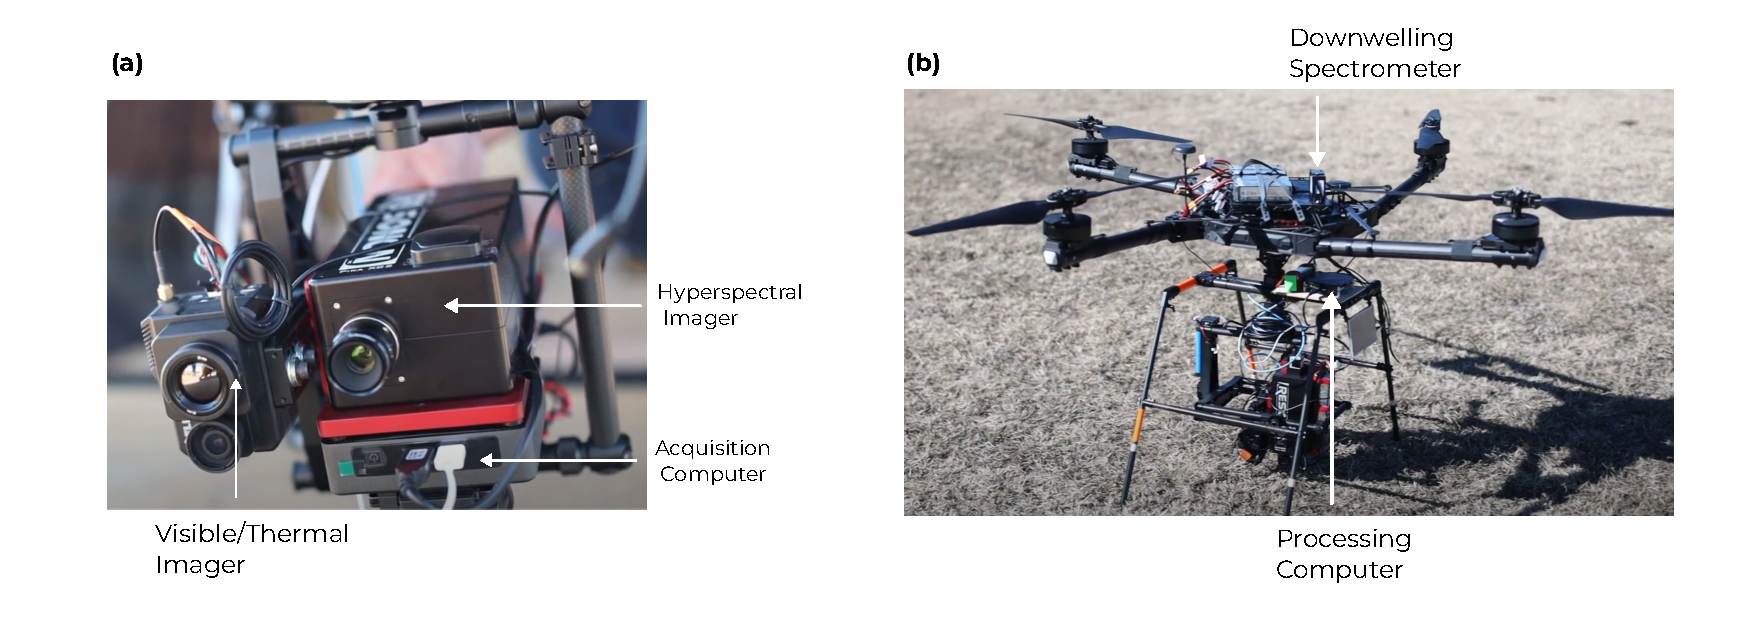
\includegraphics[width=0.9\columnwidth]{robot-team/assets/annotated-drone.pdf}
  \caption{An annotated view of the autonomous drone showcasing the hyperspectral imager and onboard compute.}
  \label{fig:uav-closeup}
\end{figure}

The aerial vehicle uses a custom built landing gear and mount made with aircraft grade aluminum and carbon fiber to carry a \href{https://resonon.com/Pika-XC2}{Resonon Visible+Near-Infrared (VNIR) Pika XC2} hyper-spectral camera (391–1011 nm) with a Schneider Xenoplan 1.4/17 mm lens, and a \href{https://www.flir.com/products/duo-pro-r/}{FLIR Duo Pro R}, (640 × 512, 25 mm, 30 Hz) combining a high resolution, radiometric thermal imager, 4K color camera, and a full suite of onboard sensors. On the top of the quad copter there is a sky facing Ocean Optics UV-Vis-NIR spectrometer measuring the incident down-welling irradiance with a 180 degree cosine corrector, allowing us to convert the raw radiance measurements of each pixel to reflectance.


%% we can discuss remote sensing, hyperspectral imaging, and the robot team here... Let's fetch some text from the 2019 paper.

%% \begin{itemize}
%% \item Remote Sensing: data acquisition, processing, and interpretation of images, and related data, obtained from aircraft and satellites that record the interaction between matter and electromagnetic radiation
%% \item Source: the source of electromagnetic radiation, e.g. the sun, black-body radiation, microwave radar, etc...
%% \item Atmospheric Radiation: The EM radiation propagating through the atmosphere. Moderated by various processes including absorption and scattering
%% \item Earth's Surface Interactions: Amount and spectral distribution of radiation emitted/reflected by the earth's surface. This depends on
%%   \begin{itemize}
%%   \item physical properties of the matter
%%   \item wavelength of EM radiation that is sensed
%%   \end{itemize}
%% \end{itemize}

%% \begin{figure}[!hbt]
%%   \centering
%%   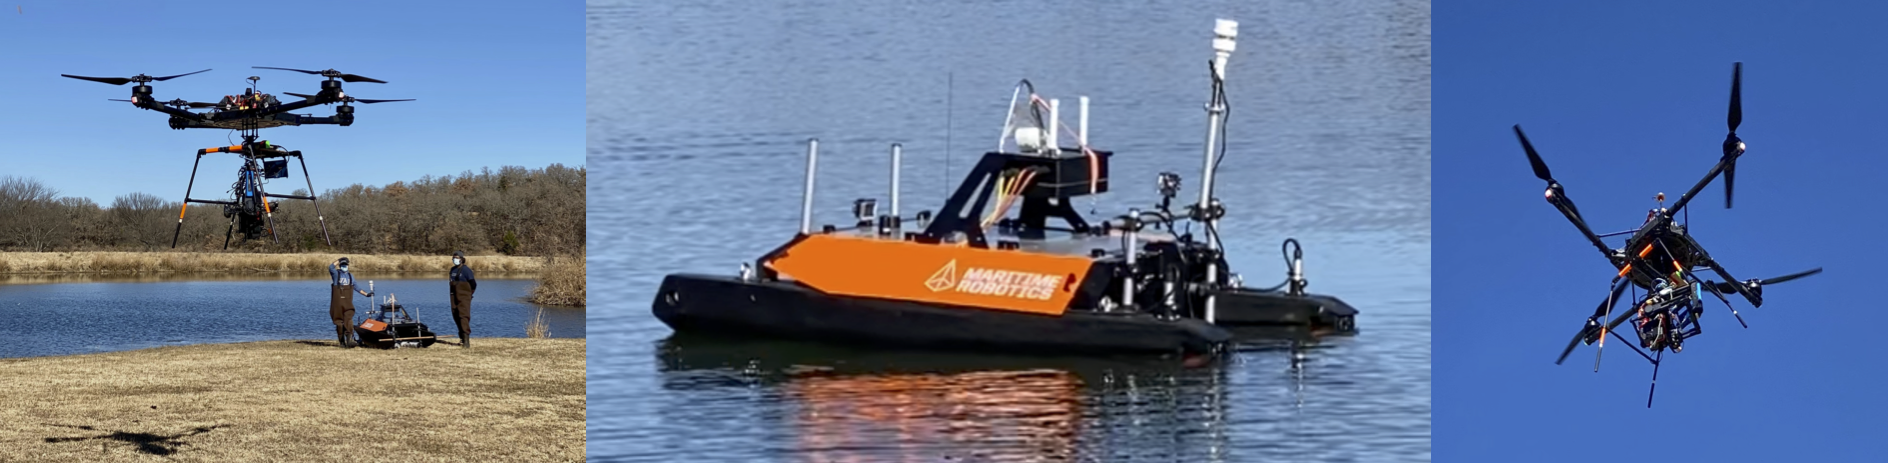
\includegraphics[width=0.85\columnwidth]{physical-sensing/Photos.png}
%% \end{figure}



% -------------------------------------------------------------------- %
\section{A Low Cost Sensor Network For Air Quality Monitoring}

The highly expensive cost to acquire, calibrate, and maintain reference grade air quality monitors makes it challenging to assess the importance of spatial and temporal variability on local air quality. Since factors such as weather, terrain, traffic, and the distribution of other sources can all effect local air quality, the development of low-cost sensing solutions is vital to address risks of poor air quality on local communities. To address this gap, we have developed a hierarchy of low-cost air quality monitors which we have deployed throughout the Dallas Fort-Worth (DFW) metroplex. In this section, we describe the relevant sensor types as well as a robust data processing and visualization pipeline developed to enable open access to high quality data.

The sensor network is comprised of a combination of two types of nodes: \textit{Central Nodes} and \textit{LoRa Nodes}. The central nodes are designed to be deployed in locations with where dedicated power is available. Each contains a variety of sensors including Particulate Matter, VOCs, $\mathrm{CO_2}$, $\mathrm{NO_X}$, ionizing radiation, incident light intensity, sound levels, as well as meteorological variables including temperature, pressure, relative humidity, and dew point. The powered Central Nodes are equipped with a cellular modem to facilitate data transfer from the field.

Each Central Node supports a collection of ~10 LoRa nodes (named for the LoRa long rage wireless transmission protocol) which can be separated by distances up to ~5 km or more if line of sight is established. These smaller sensors are self powered using a combination of battery and solar cells, and each measures a similar array of relevant air quality metric including particulate matter concentrations, gas concentrations, and meteorological parameters. Designs for the two node types are illustrated in Figure {fig:mints-nodes}.
\begin{figure}[!hbt]
  \begin{subfigure}{.5\textwidth}
    \centering
    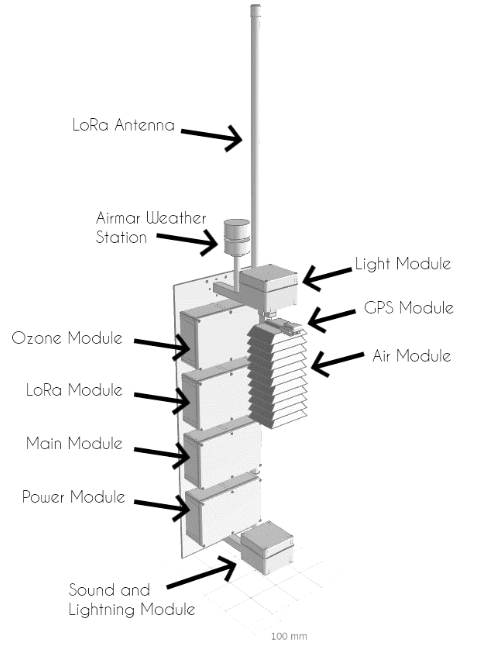
\includegraphics[width=.8\linewidth]{physical-sensing/central-node.png}
    \caption{A 3d model of a Central Node}
  \end{subfigure}
  \begin{subfigure}{.5\textwidth}
    \centering
    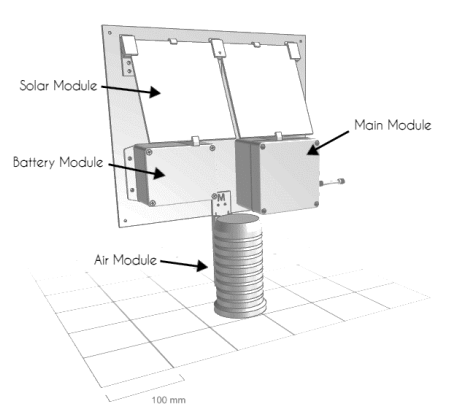
\includegraphics[width=.8\linewidth]{physical-sensing/lora-node.png}
    \caption{A 3d model of a LoRa Node}
  \end{subfigure}
  \caption{Two types of nodes from the MINTS Air Quality network.}
  \label{fig:mints-nodes}
\end{figure}

Using the LoRaWAN protocol, the Central and LoRa nodes form a low power, wide area network by which data packets from each LoRa node are transmitted in real time to the nearest Central Node. Using their inbuilt cellular connection, the central nodes are then able to pass sampled data to a data processing backend using an MQTT publish-subscribe model. As the primary goal of this network is to provide detailed, real-time air quality data, we have developed a public facing website, \url{http://SharedAirDFW.com}, to visualize the current and historic measurement at each sensor location together with 6-hour wind forecasts from NOAA and weather radar. Figure \ref{fig:sharedair-site} shows a sample screenshot of the site.
\begin{figure}[!hbt]
  \centering
  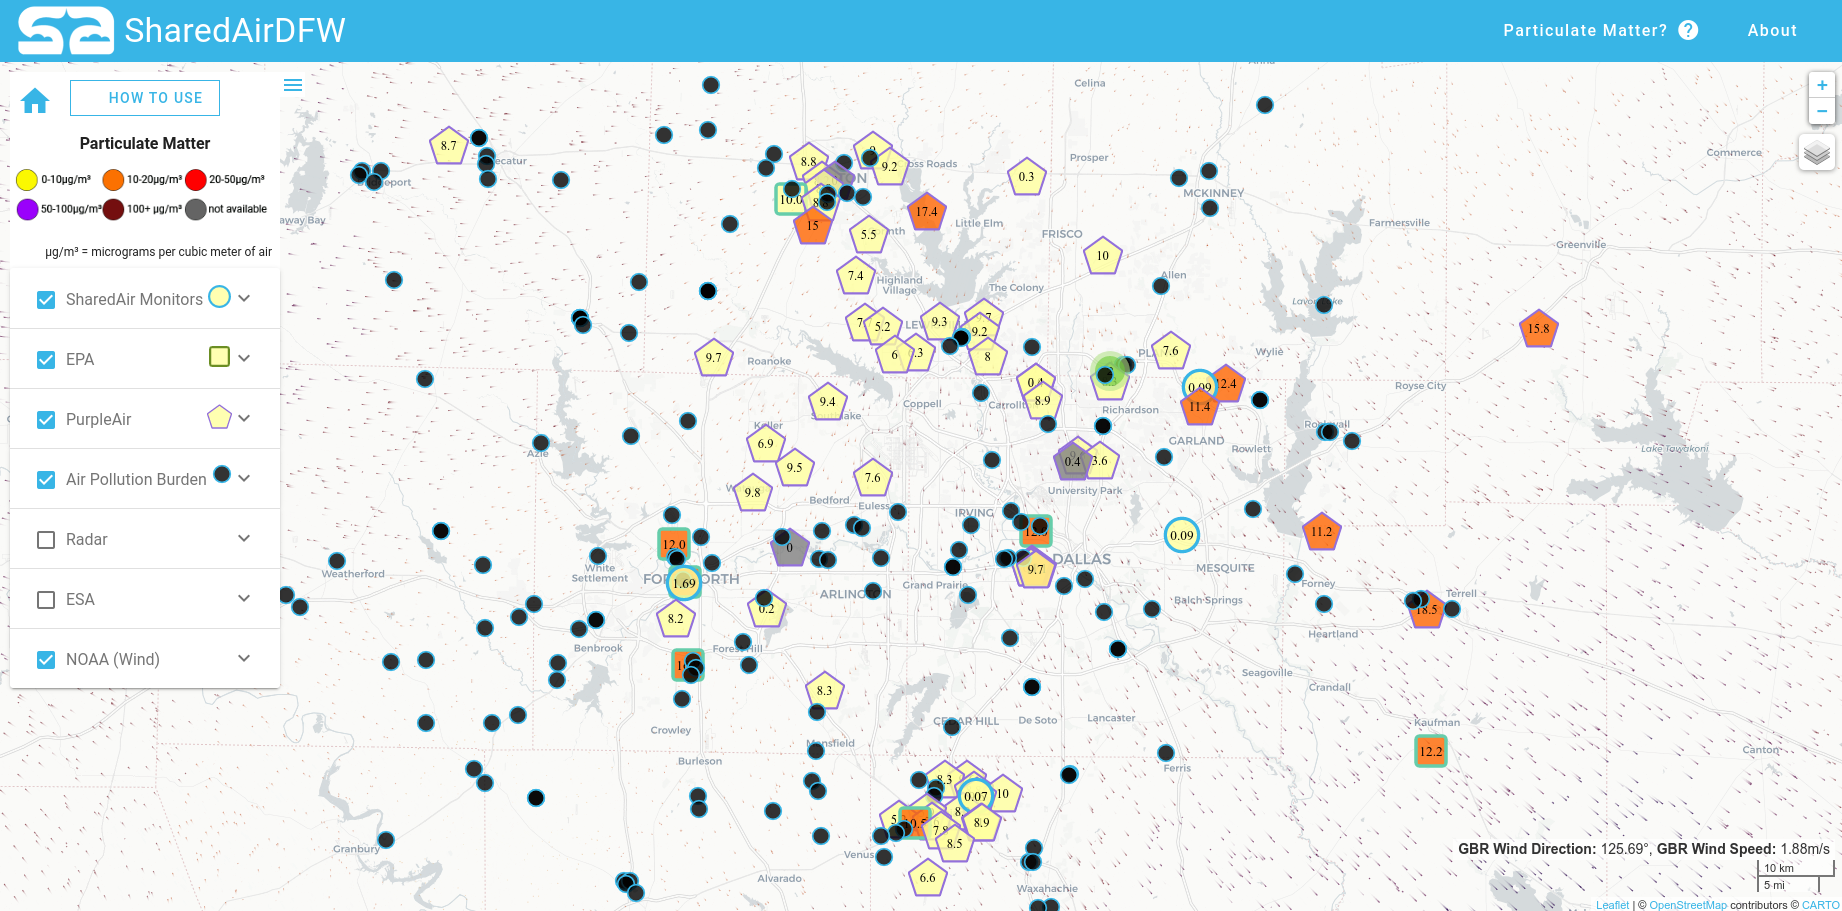
\includegraphics[width=0.85\columnwidth]{physical-sensing/sharedairdfw-homepage.png}
  \label{fig:sharedair-site}
  \caption{The interactive SharedAirDFW website show casing real time data streams from the MINTS sensor network.}
\end{figure}

In order to automate data collection, processing, analysis, and long-term storage, a containerized pipeline was developed as illustrated in Figure \ref{fig:dashboards}.
\begin{figure}[!hbt]
  \begin{subfigure}{.2\textwidth}
    \centering
    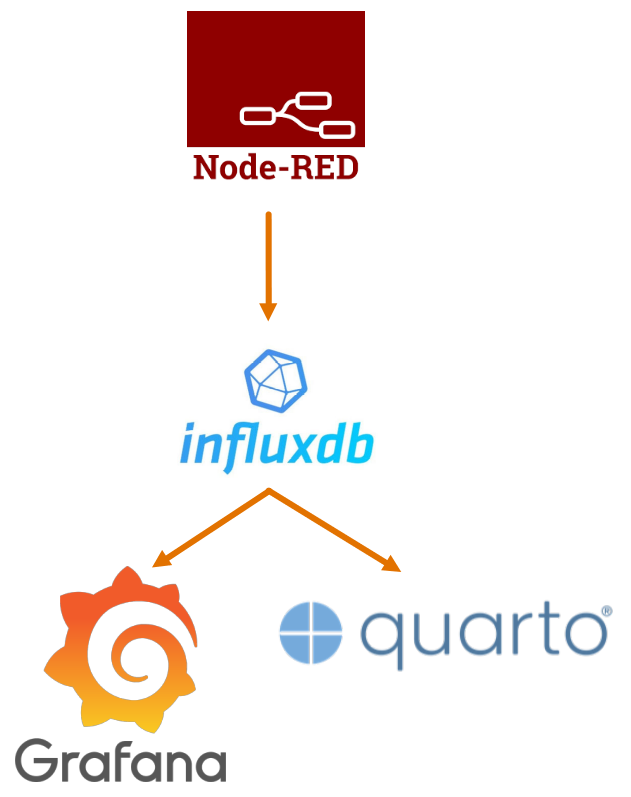
\includegraphics[width=0.85\columnwidth]{physical-sensing/docker-elements.png}
    \caption{}
  \end{subfigure}
  \begin{subfigure}{.8\textwidth}
    \centering
    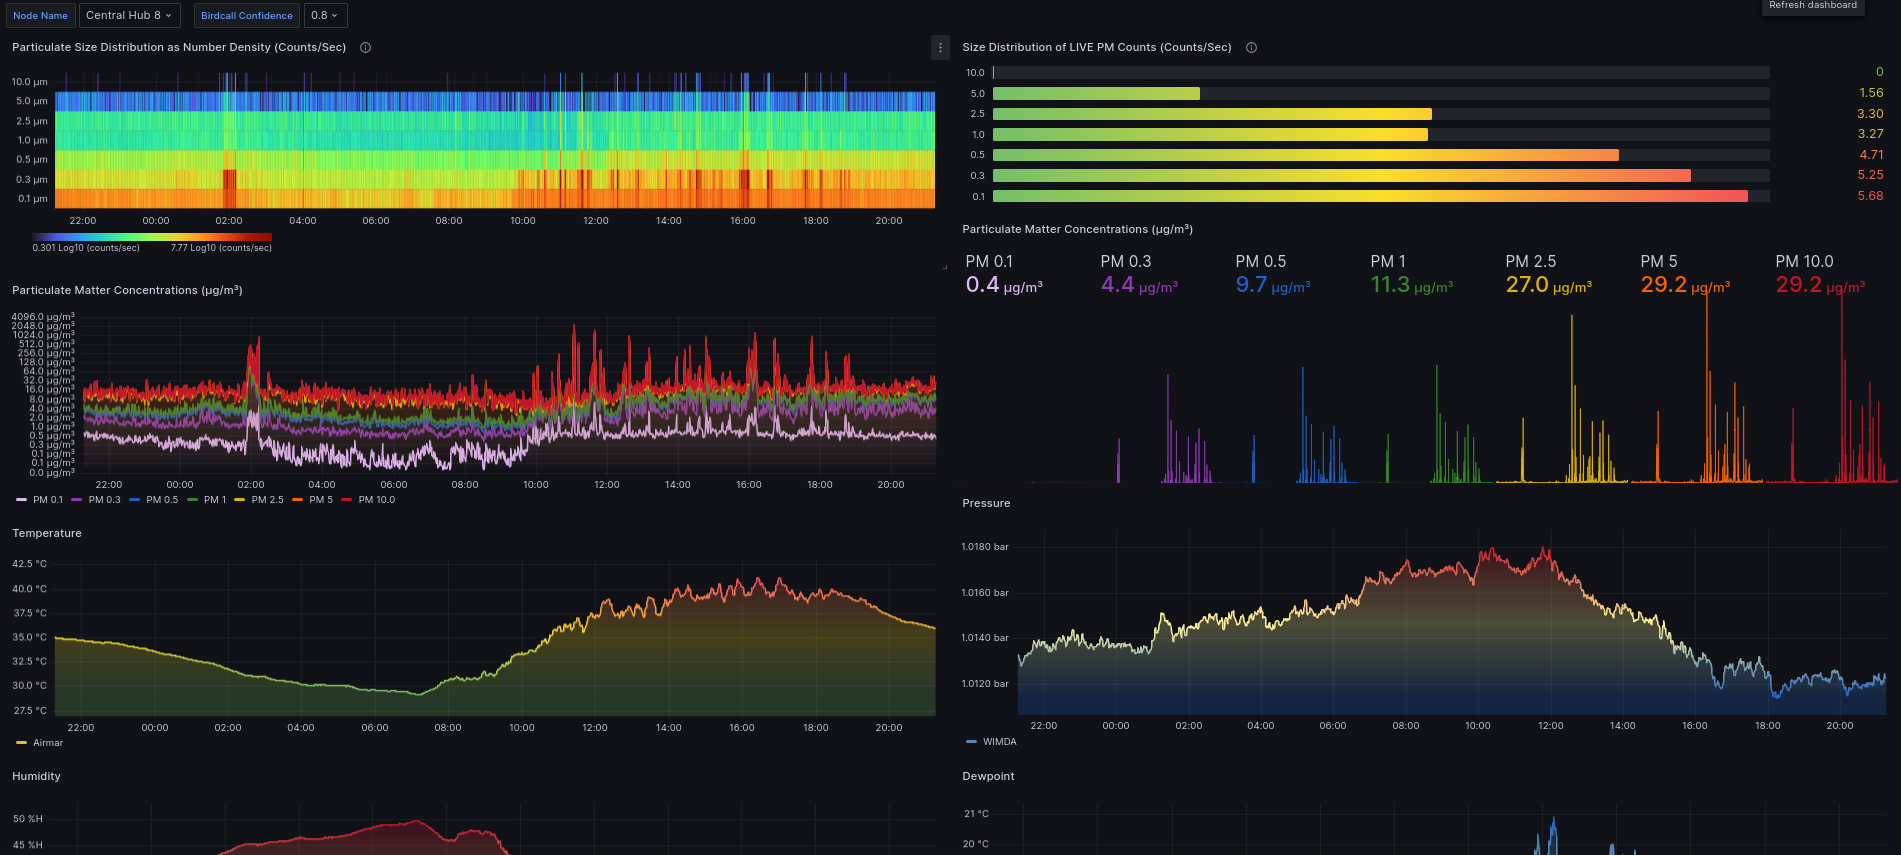
\includegraphics[width=.8\linewidth]{physical-sensing/grafana-dashboard-1.png}
    \caption{}
  \end{subfigure}
  \caption{The backend infrastructure developed to support the MINTS sensor network.}
  \label{fig:dashboards}
\end{figure}
This pipeline is composed of 5 tools at utilizes containerization for reliable development and deployment.
\begin{itemize}
\item \textbf{NodeRed}: This tool developed by IBM allows the creation of complex data processing pipelines by defining directed acyclic graphs (DAGs) composed of individual processing nodes. We utlize this tool to subscribe to each sensor's relevant MQTT topic and decode the data packets into the relevant sensor measurements. At the end of each sensor pipeline, the data are then injected into the InfluxDB time series database. A key advantage of NodeRed is that the wide array of pre-existing nodes enables a no-code solution that easy to maintain.
\item \textbf{InfluxDB}: This is a open source time series database optimized for large cardinality datasets. By storing processed data in InfluxDB, we are able to provide easy queryable access to real time and historic data.
\item \textbf{Grafana}: This tool is an open source visualization platform for creating interactive dashboards. We utilize Grafana to create detailed, real-time displays for each sensor in the network that we can use to observe \textit{all} incoming measurements as well as identify pollution events and monitor sensor status.
\item \textbf{Quarto}: This tool allows the generation of automated analysis reports by using a literate programming paradigm built on top of Jupyter Notebooks. By using quarto we are able to automatically perform daily, weekly, monthly, and annual analyses for each sensor in the network and collect the results into formatted PDFs or a static website. We are developing analysis using quarto together with Julia, Python, and R to facilitate detailed report generation and provide actionable insights.
\item \textbf{Open Storage Network}: With help from Dr. Chris Simmons, we have developed a pipeline for long term data storage utilizing the Open Storage Network to provide open access to historic sensor data stored in the popular S3 format.
\end{itemize}
Individual sensor dashboards are made publicly available at \url{http://mdash.circ.utdallas.edu:3000}. Historic data are updated daily at \url{https://portal.osn.xsede.org/s3browser//?bucket_path=https://ncsa.osn.xsede.org/ees230012-bucket01}.


% -------------------------------------------------------------------- %
\section{Reference Grade Assesment of Indoor Air: The Heart Chamber}

The coordinated Robot Team allows us to rapidly characterize novel outdoor environments with a particular focus on assessing concentrations of chemicals-of-concern in bodies of water. Our low-cost sensing network enables high spatio-temporal resolution of air quality dynamics for outdoor air. In this final section, we describe a comprehensive testing chamber for the assessment of \textit{indoor} air. This chamber, called \textit{HEART} for holistic environmental aerosol and reactive component testing, is being developed to enable assessment of the detailed chemical and aerosol dynamics which effect indoor air quality. Figure \ref{Figure.HEART-Details} provides visual overview of the design.

\begin{figure}[!hbt]
  \centering
  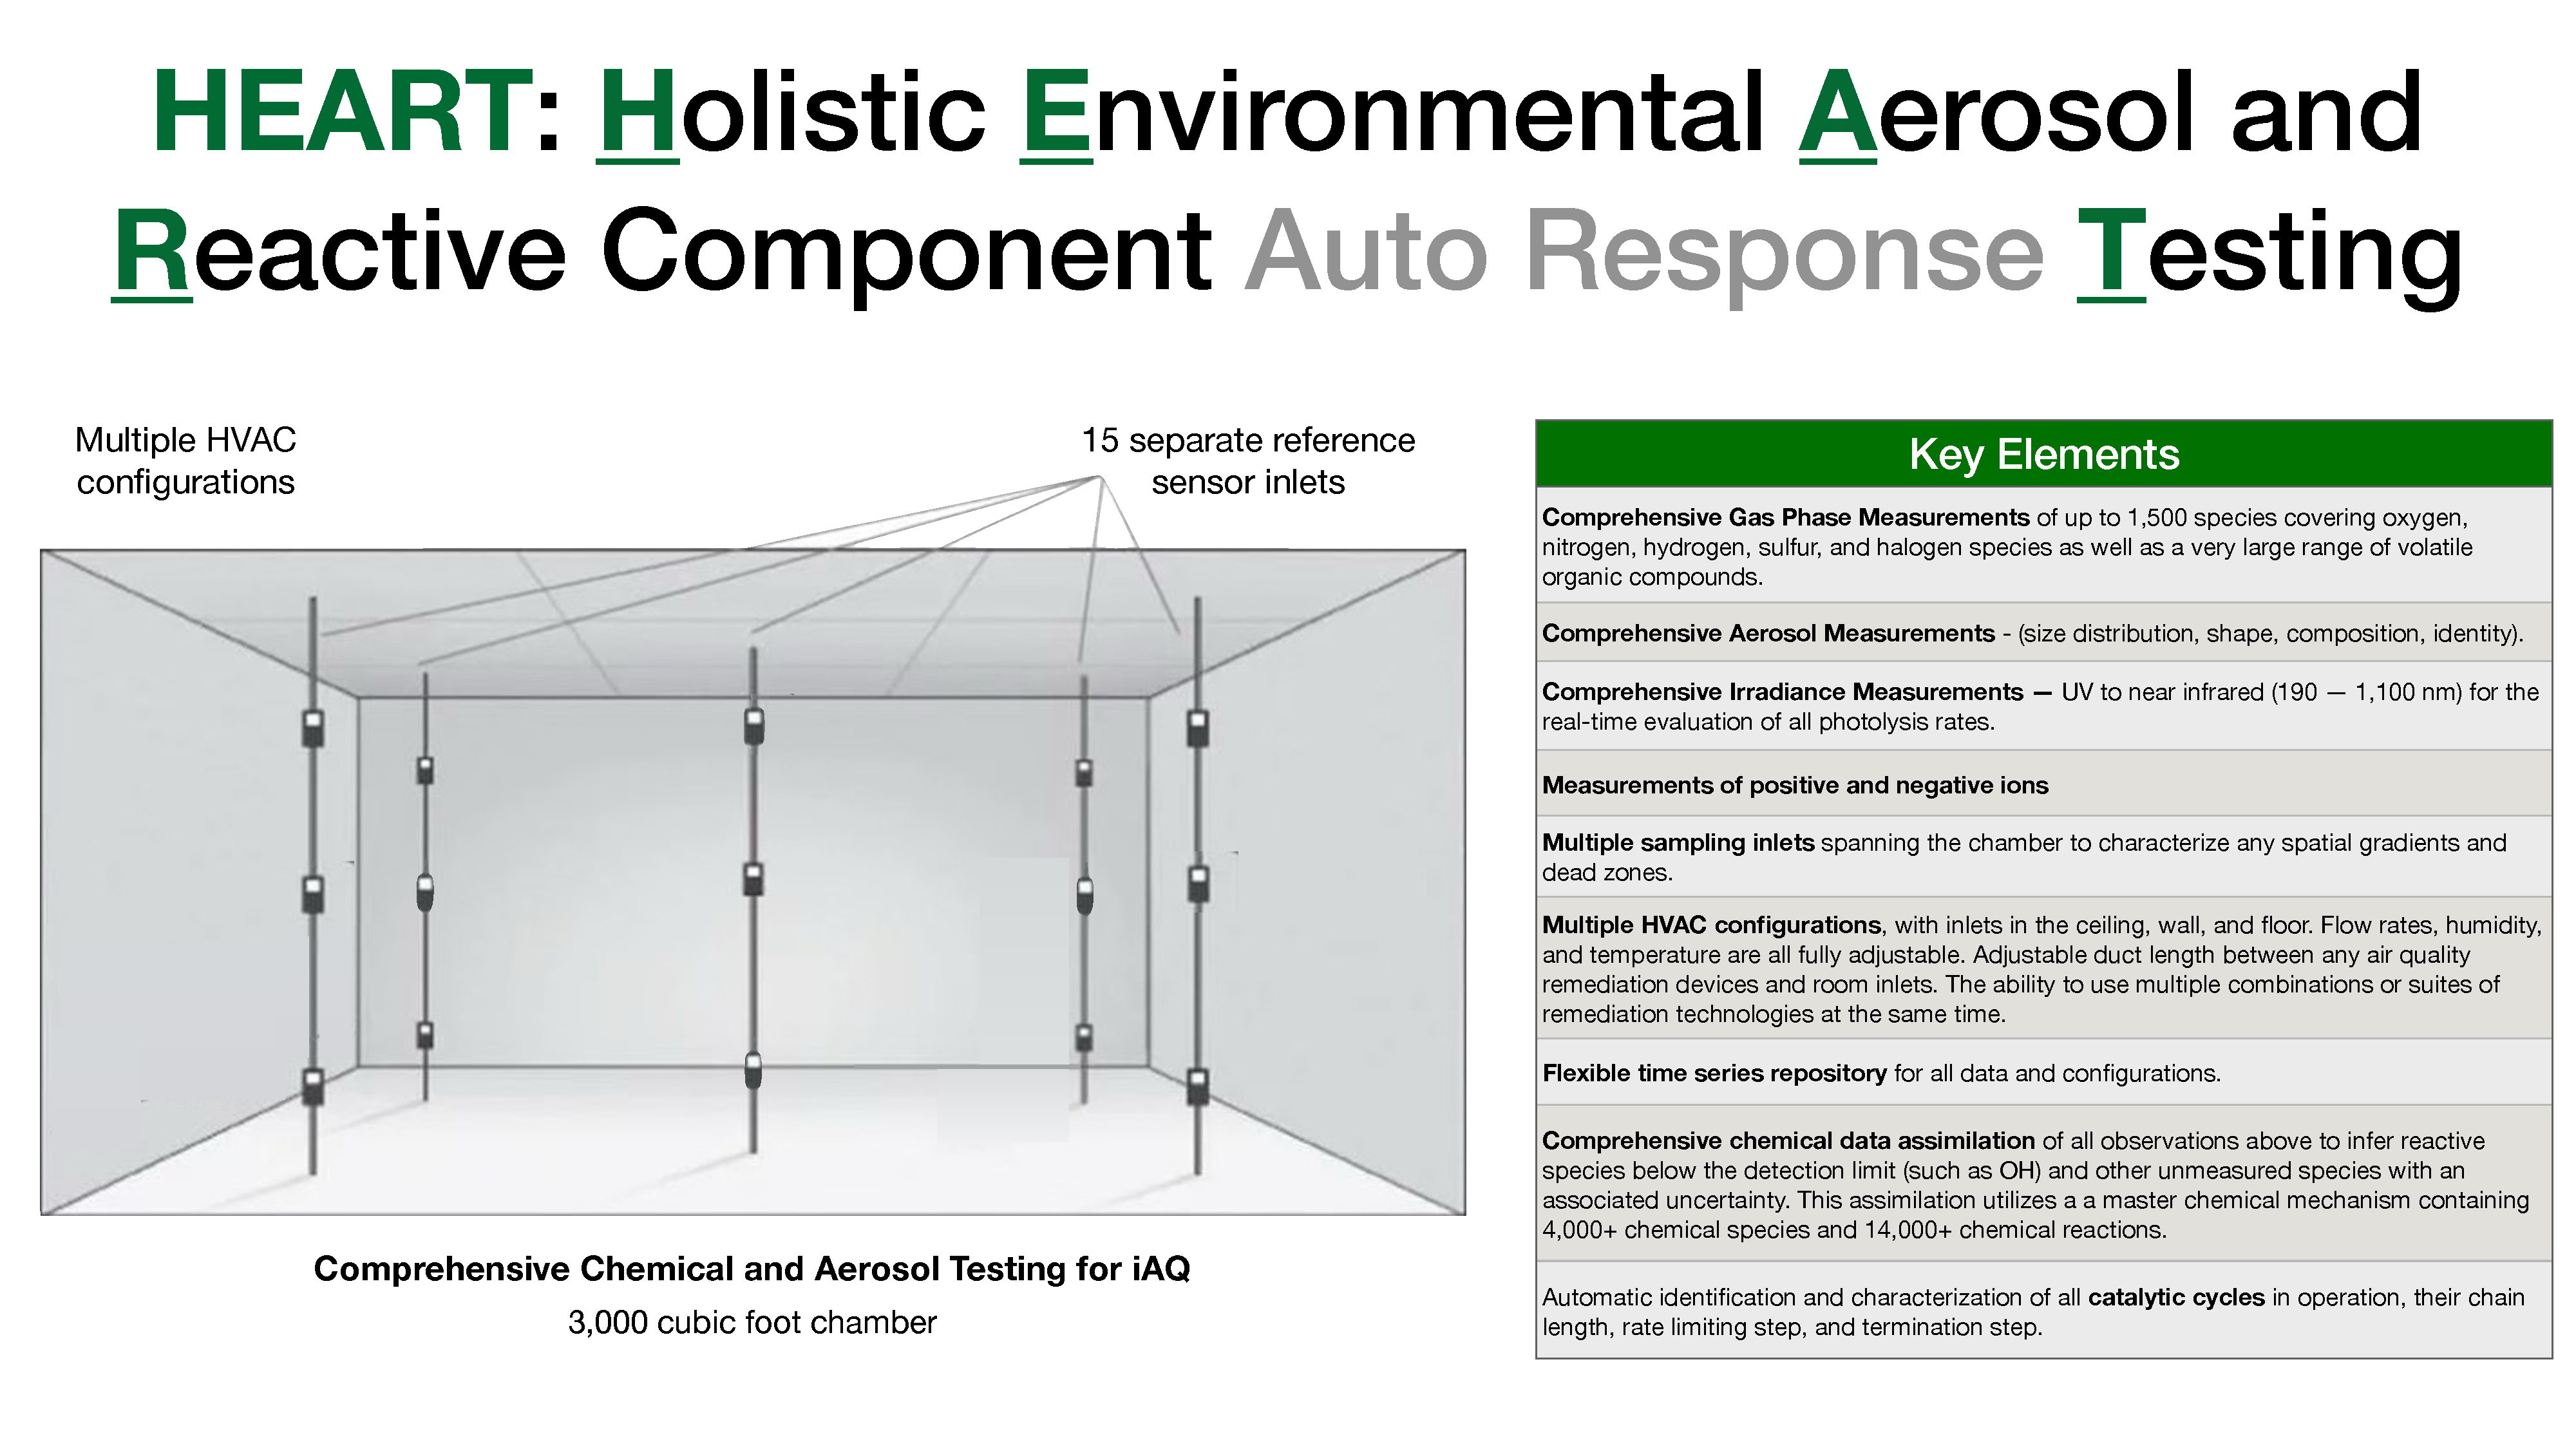
\includegraphics[width=\textwidth]{introduction/HEART-Details.pdf}
	\caption{Design of comprehensive chemical and aerosol testing for IAQ using HEART: Holistic Environmental Aerosol and Reactive Component Auto Response Testing.}
	\label{Figure.HEART-Details}
\end{figure}

The HEART test chamber is designed for comprehensive characterization of air quality including the chemical composition (characterizing hundreds of chemicals), positive and negative ion density, aerosol size (from 5 nm to 100 microns), detailed morphology (shape), and composition, and individual bio-aerosol particle recognition, along with the accurately characterized illumination environment characterized in more than 4,000 wavelengths from the UV to the near-infrared (190 — 1,100 nm) using a NIST calibrated spectrometer. The lighting environment is important, as, after all, air quality is atmospheric photochemistry in the indoor built environment. Photolysis is a key driver. Furthermore, some of the frequently advocated families of remediation technologies make use of various parts of the ultraviolet spectrum. This high-energy region of the spectrum has important implications for indoor air quality.

\begin{figure}[h]
  \centering
  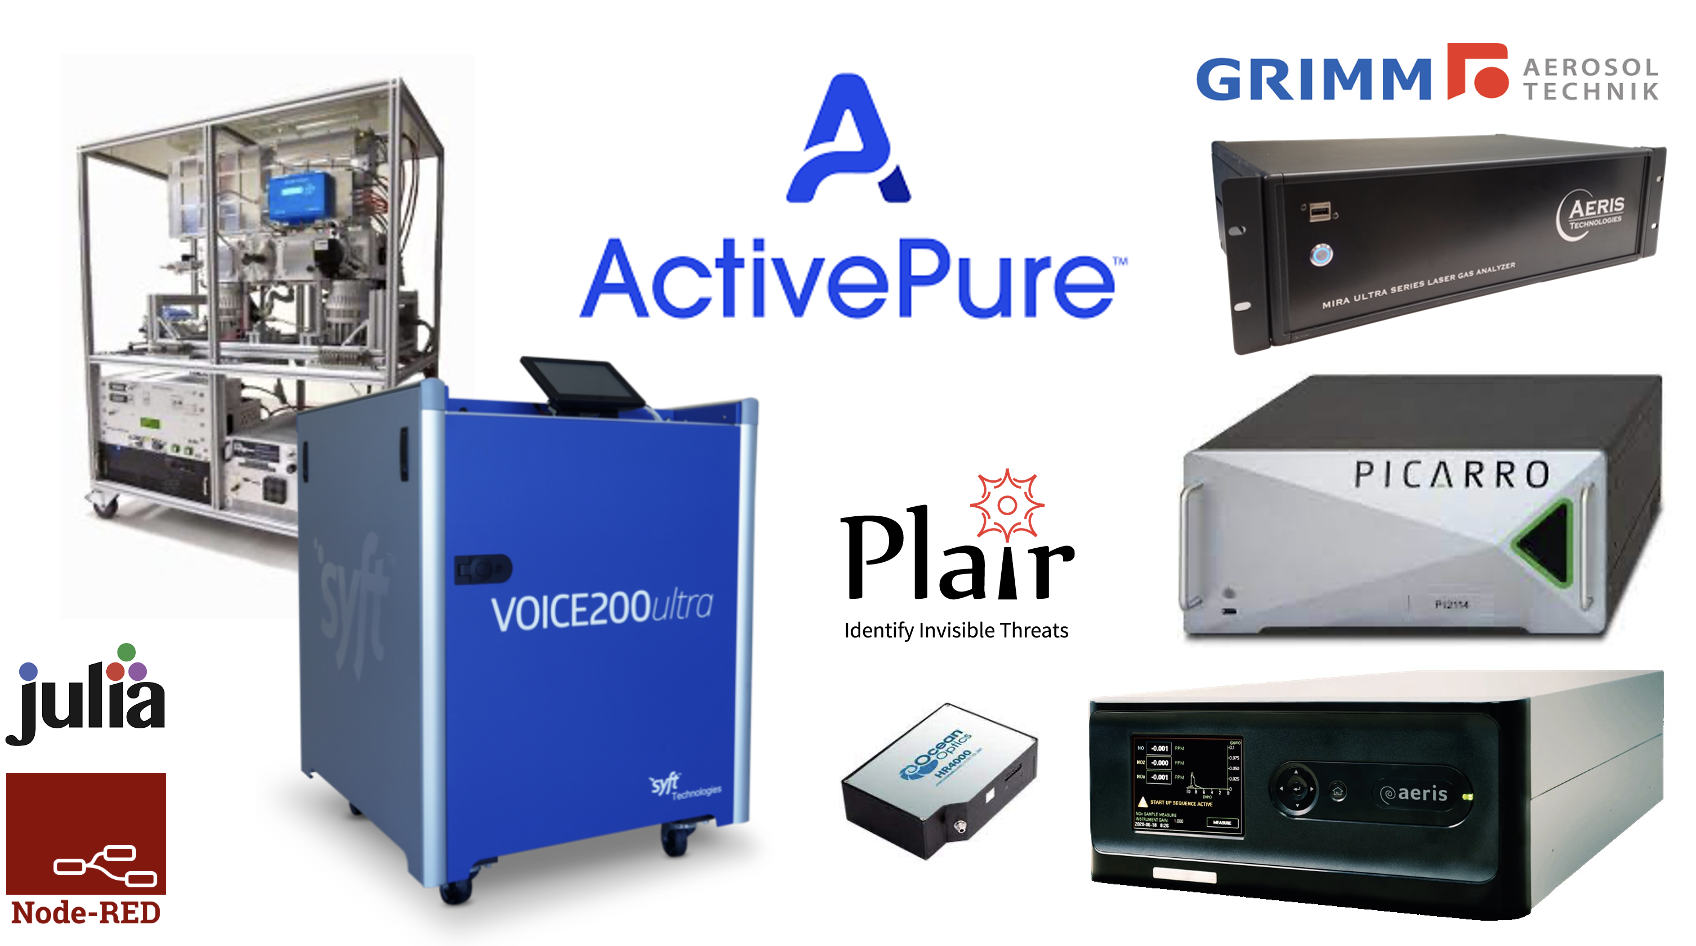
\includegraphics[width=\textwidth]{introduction/LabOverview.png}
	\caption{Visual overview of the various infrastructure components of the ActivePure lab. Note that the lab uses multiple instruments of those shown to accommodate the stated range of analytes.}
	\label{Figure.InstrumentOverview}
\end{figure}
As shown in figure \ref{Figure.InstrumentOverview}, 15 inlets in the HEART chamber are sampled using a combination of instruments including an Aerodyne Aerosol Mass Spectrometer (AMS), a Selected Ion Flow Tube (SIFT) mass spectrometer, a collection of gas concentration analyzers, as well as a an Ocean Optics HR4000 UV-NIR spectrometer, and a GRIMM wide range aerosol spectrometer. In the spirit of \textit{multi-use}, the NodeRed+InfluxDB+Grafana software stack are also utilized to log sensor measurements directly into a time series database with real time dashboards for monitoring of experiments.

It is inevitable that some chemical species, for example, reactive components such as $\mathrm{OH}$, will typically be below the detection limit of the measurement systems. Information on these unmeasured reactive components is naturally embedded in the shape of the time-series observations of the chemical species they are reacting with and in the partitioning between the large number of measured components that they are reacting with. This information can be effectively extracted, together with associated uncertainty estimates, using chemical data assimilation \cite{ISI:A1995TA29300008, Lary1999a, Lary2003a}. Hundreds of chemicals measured in real-time in the HEART chamber, along with high-resolution irradiance spectra used to calculate real-time photolysis rates and real-time aerosol measurements, are assimilated in a full chemical data assimilation system with a detailed chemical mechanism.



% -------------------------------------------------------------------- %

%% \section{Hyperspectral Imaging}

%% The following are notes from the Manolakis textbook that I originally kept \href{https://github.com/john-waczak/dissertation/blob/main/notes/remote_sensing/Manolakis/Introduction.md}{here}. NOTE: we will need to either make new figures or correctly cite these for attribution.

%% \subsection{Hyperspectal Imaging Sensors}

%% \begin{itemize}
%% \item \textit{Hyperspectral Sensors} aka imaging spectrometers
%%   \begin{itemize}
%%   \item scanning mechanism
%%   \item imaging system
%%   \item spectrometer
%%   \end{itemize}
%% \item 3 types of resolution
%%   \begin{enumerate}
%%     \item spatial
%%     \item spectral
%%     \item radiant
%%     \item (temporal?)
%%   \end{enumerate}
%% \end{itemize}

%% \subsection{Spectral-Spatial Data Collection and Organization}
%% Data collected into \textit{datacube} with 2 spatial dimensions, 1 spectral dimension

%% \begin{figure}[h]
%%   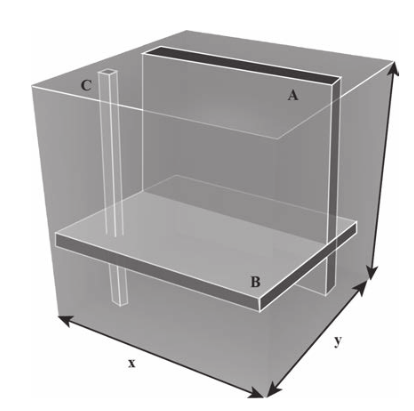
\includegraphics[width=10cm]{datacube.png}
%% \end{figure}

%% \begin{figure}[h]
%%   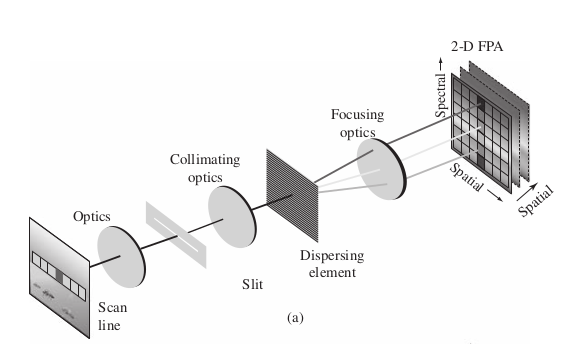
\includegraphics[width=10cm]{pushbroom.png}
%% \end{figure}


%% Different types of rigs:
%% \begin{itemize}
%%   \item Pushbroom scanner (ours)
%%   \item Staring System
%%   \item Fourier Transform Imaging Spectrometer (FTIS)
%% \end{itemize}


%% \subsection{Spatial Sampling}
%% \begin{itemize}
%%   \item ground resolution elements are mapped to picture elements (pixels)
%%   \item IFOV: Instantaneous Field of View
%%   \item Cross track dimension: the projection of the long axis of the slit (i.e. the axis of the pushbroom sensors)
%%   \item Along track dimension: the direction accumulated by traveling
%%   \item Ground Sample Distance: physical size of projected pixel element
%% \end{itemize}


%% \begin{figure}[h]
%%   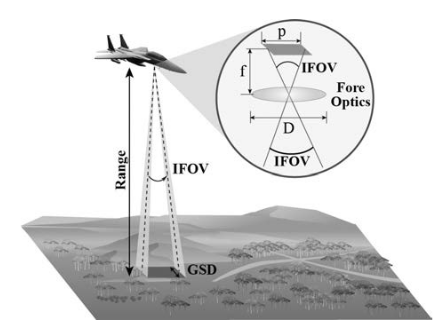
\includegraphics[width=10cm]{scanningProcedure.png}
%% \end{figure}


%% \subsection{Spectral Sampling}
%% \begin{itemize}
%%   \item Recovery of spectral info is imperfect due to finite sampling
%%   \item Spectral Response Function: is the weighing function that describes the wavelengths that are transmitted to a particular spectral sample
%% \end{itemize}

%% \subsection{Radiometric Sampling}
%% \begin{itemize}
%%   \item detector transforms  radiant power to electrical signal
%%   \item electrical signal converted to number via analog-to-digital converter
%%   \item photon detectors
%% \end{itemize}

%% \subsection{Signal Considerations}
%% Strength of signal is determined by:
%% \begin{itemize}
%%   \item Terrain composition affects amount of radiant energy reflected/emitted from ground resolution element
%%   \item Range: Intensity drops off by inverse square law. Further you are away, the worse the signal
%%   \item Spectral Bandwidth: output signal of detector element is proportional to spectral bandwidth of the detector
%%   \item Instantaneous Field of View: Decreasing IFOV increases spatial resolution but weakens the signal
%%   \item Dwell Time: the time required to sweep the IFOV across the ground resolution element, i.e. the time-on-pixel. Longer dwell time $\to$ more accumulated photons $\to$ more signal.
%% \end{itemize}





%% % -------------------------------------------------------------------- %

%% \section{Remote Sensing}

%% mention different types of satellite data platforms (mostly optical), differences in orbits, coverage, etc... Also good to discuss the increasing use of drones for a variety of applications including intelligent agriculture, geophysics, mapping, etc...



%% \subsection{Infrared Sensing Phenomenology}

%% Main passive sources of EM radiation for remote sensing are light emitted by the sun and the self-emission via black-body radiation of objects due to their temperature.

%% \subsection{Sources of Infrared Radiation}
%% \begin{itemize}
%% \item \textbf{spectral radiant exitance} power per unit area emitted by the sun. We can treat this as a black body with temperature $5800 K$, maximum emittance at $\lambda = 0.50$ $\mu m$.
%% \item The Earth is ~$300 K$ with maximum spectral radiant emittance at $\lambda = 9.7$ $\mu m$. This is known as the \textbf{thermal infrared}
%% \end{itemize}

%% \subsection{Atmospheric Propagation}

%% \begin{itemize}
%% \item Key parameter is the \textbf{path length} of atmosphered traveled through before it arrives at the remote sensing system. Main effects are:
%%   \begin{itemize}
%%   \item \textbf{Atmospheric Scattering}: diffusion of radiation by particles in the atmosphere
%%   \item \textbf{Absorption}
%%   \end{itemize}
%% \item Useful remote sensing spectral regions are obtained via the \textbf{Transmission Spectrum}.
%%   \begin{itemize}
%%   \item \textbf{Reflective Range}: $0.35-2.5$ $\mu m$. Dominated by solar illumination
%%   \item \textbf{Water Absorption}: $0.2-2.5$ $\mu m$.
%%   \end{itemize}
%% \item \textbf{Atmospheric Windows}: Regions of low atmospheric absorption
%% \end{itemize}

%% \subsection{Reflectance and Emissivity Spectra}

%% There are three processes that occur when EM radiation meets and interface:
%% \begin{enumerate}
%%   \item \textbf{Reflection}: Solar illumination dominates here. Consequently, this part of the spectrum is used to characterize the surface
%%     \begin{itemize}
%%     \item \textbf{Specular Reflectors}: Flat surfaces that act like mirrors, i.e. $\theta_i = \theta_r$.
%%     \item \textbf{Diffuse (Lambertian) Reflectors}: Rough surfaces that reflect uniformly in all directions.
%%     \item \textbf{Real Reflectors}: Somewhere between the specular and diffuse.
%%    \end{itemize}
%% \item \textbf{Absorption}
%% \item \textbf{Transmission}
%% \end{enumerate}

%% \begin{itemize}
%% \item Fractions vary as a function of $\lambda$
%% \item Remote sensing usually cares about \textit{diffuse} reflectors because this is the dominant type of most materials (water being an exception).
%% \item Reflectance of a material is characterized by its \textbf{Reflectance Spectrum}, that is, the percent of incident light reflected as a function of wavelength.
%%   \begin{itemize}
%%   \item Dips in reflectance spectrum are called \textbf{absorption features}
%%   \item Peaks are called \textbf{Reflectance Peaks}
%%   \end{itemize}
%% \item \textbf{Emissivity Spectrum}: The ratio of radiant emittance at a given temperature to the radiant emittance of a black body at the same temperature.
%% \end{itemize}


